\documentclass[a4paper, 12pt]{article}
\usepackage{titling}
\usepackage[margin=3.0cm]{geometry}
\usepackage{graphicx}
\usepackage{amsmath}
\usepackage{amssymb}
\usepackage{lipsum}

\usepackage[style=ieee, url=false, doi=false, isbn=false]{biblatex}
\addbibresource{bibliography.bib}

\begin{document}

\title{\bf Random Features and the Jamming Transition in Artificial Neural Networks}
\author{
    % Hudson Cooper\\ % REDACT FOR SUBMISSION
    King's College London\\
    M.Sc.\ in Complex Systems Modelling
}
\date{\today}

\begin{titlingpage}
\maketitle
\begin{abstract}
\lipsum[1]
\end{abstract}
\end{titlingpage}

\section{Introduction}
Neural networks are one of the most highly successful classes of models in modern machine learning. While there is a rich body of literature which empirically examines the ability of neural networks to fit to and generalize from data, the field is lacking a cohesive theoretical framework for designing these networks and for understanding their incredible success. \\

\subsection{Motivation}

Until recently, one of the most poorly understood features of modern neural networks is their operation in a regime that is seemingly at odds with the bias-variance trade-off, a main tenet of classical statistical learning. The bias-variance trade-off implies that more expressive models are likely to find spurious patterns in data, and therefore practitioners should seek to build models that are ``as simple as possible, but no simpler." Neural networks, however, typically operate in an extremely over-parameterized regime, containing many more parameters than there are data. Neural networks have been shown to be so highly expressive that they are able to interpolate data and perfectly classify training data, even when labels have been replaced with pure noise \cite{zhangUnderstandingDeepLearning2017}. Despite their complexity and extreme expressiveness, they are able to generalize extremely well in practice, often outperforming classical models on test data. \\

Recent work \cite{belkinReconcilingModernMachine2019} has characterised this phenomena in terms of the so-called ``double-descent" curve, which is visually represented in figure \ref{doubledescent}. Two distinct regimes of model complexity are separated by the interpolation threshold, the point at which models are able to obtain perfect performance on training data at the cost of extremely high test error. To the left of this threshold is the under-parameterized regime, in which the classical bias-variance trade-off holds. As model complexity increases, generalization error follows a U-shaped curve, decreasing to a minimum before increasing to a peak at the interpolation threshold, where classical ``overfitting" occurs. To the right of this threshold, however, the generalization error again decreases. The global optimum often occurs deep in the over-parameterized regime, sometimes in the limit of ``infinite" complexity. This double-descent phenomenology is far from unique to neural networks, and it has been observed in other contexts, for example in random forests, random feature models, and kernel machines \cite{ belkinReconcilingModernMachine2019, belkinUnderstandDeepLearning2018}.\\

\begin{figure}[ht]
\centering
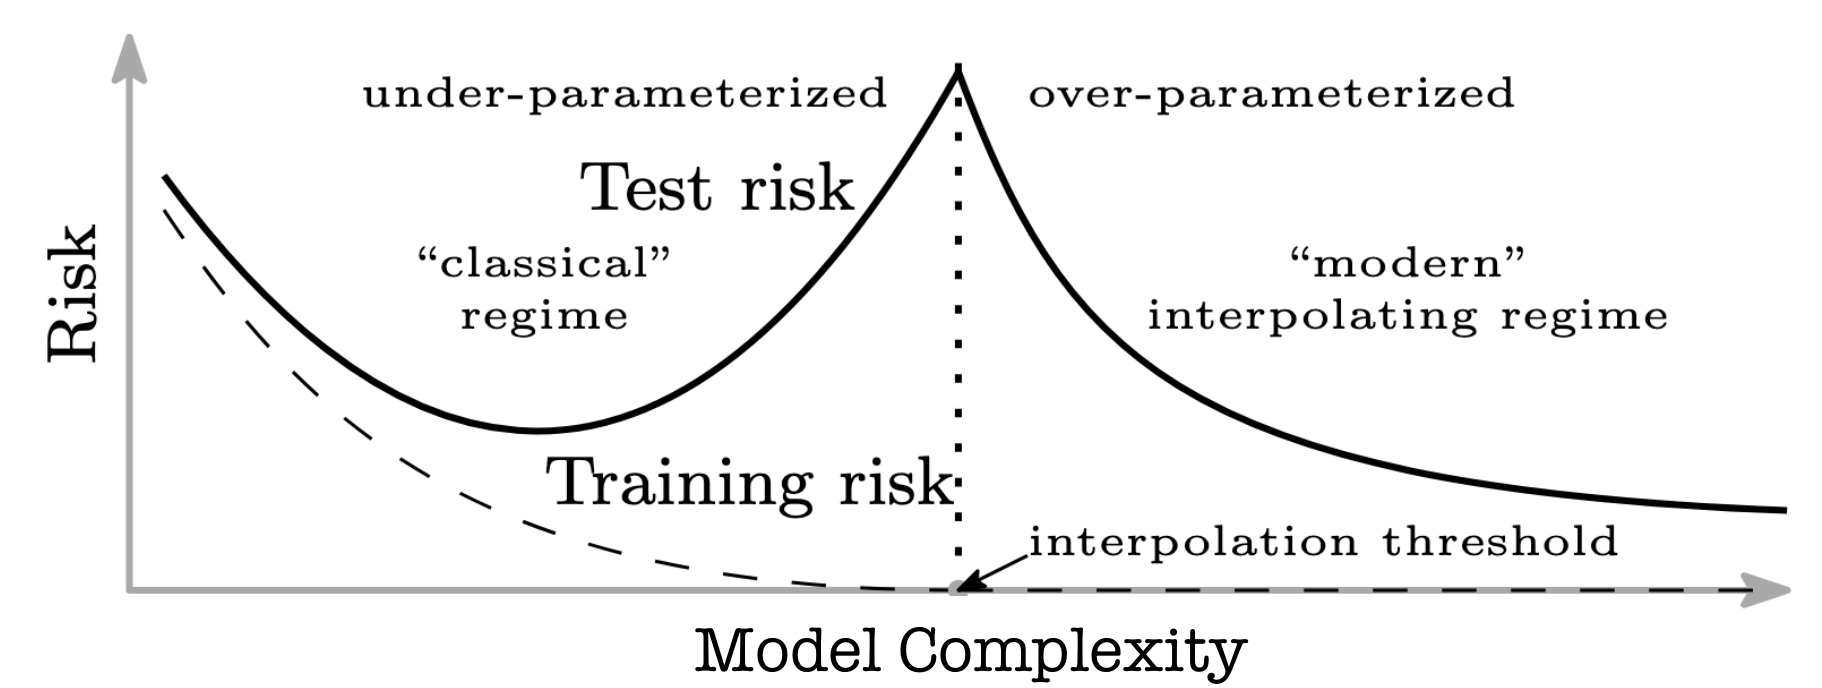
\includegraphics[width=0.7\textwidth]{docs/assets/double_descent_reconciling.png}
\caption{Visual depiction of the double descent curve, adapted from \cite{belkinReconcilingModernMachine2019}. The ``classical" U-shaped bias-variance trade-off is seen in the under-parameterized regime to the left of the interpolation threshold, and a second descent is seen in the over-parameterized regime to the right. Training error (``risk'') is represented with a dashed line, and test error is represented with a solid line.}
\label{doubledescent}
\end{figure}


Study in \cite{baity-jesiComparingDynamicsDeep2019} and \cite{geigerJammingTransitionParadigm2019} of the training dynamics of neural networks undergoing stochastic gradient descent (SGD)  has revealed deep qualitative similarities between the interpolation threshold and the ``jamming" phase transition in granular solids. By appealing to analogies between the physical phenomena of jamming and the separation of the under- and over-parameterized regimes by the interpolation threshold in neural networks, \cite{geigerJammingTransitionParadigm2019} and \cite{spiglerJammingTransitionOverparametrization2019} predict and empirically test a characterization of the training dynamics near and beyond the threshold. 

TODO: More here. What are the analogies? 

\subsection{Goals and Roadmap}

The goal of this paper is to examine a recently popular model for understanding neural networks, the "random features" model. The random features model displays the characteristics of double descent independently of the training dynamics used. We therefore explore whether the jamming phenomenology is recovered by the random features model and the extent to which feature learning plays a role in its emergence.\\


Still poorly understood:\\
- why, when, and how feature learning improves generalization\\
- how the location of the interpolation threshold is affected by feature learning\\
- how the ability of a network to build quality features depends on architecture (and relationship to inductive bias) \\
- double descent: a property of dynamics or a property of features?\\
- the role that feature learning plays in the emergence of the jamming phenomenology\\

This paper will conduct a review of... and then explain the novel contributions, then... OUTLINE GOES HERE

\section{Background}
\subsection{Deep Learning, Random Features, and Kernel Methods}

Recent study of neural networks in the infinite-with limit has shown that under gradient-descent on the network parameters, the outputs follow the kernel gradient of the loss functional with respect to the ``Neural Tangent Kernel" (NTK) \cite{jacotNeuralTangentKernel2018}. For a particular scaling choice of the final layer weights, the NTK converges to a deterministic limit that depends only on the network architecture, is independent of parameter initialization, and is fixed throughout training. This scaling choice has been dubbed the ``lazy learning regime" due to this invariance. Experimental evidence showed a good agreement between the limiting kernel and networks trained in the large but finite width setting, and further work in \cite{allen-zhuConvergenceTheoryDeep2019} formalized this connection by showing that overparameterized networks of finite width converge to a global optimum given by the NTK.\\

The lazy learning regime admits an alternative representation in which the network outputs at any time during training can be expressed as a first-order Taylor expansion of the network about its initial weights \cite{leeWideNeuralNetworks2019}. In other words, networks in the lazy-learning regime are linear models of random features gien by the gradient of the network with respect to its parameters at initialization. For a network $f_\theta$ with initial parameters $\theta_0$ and an initialization such that $f_{\theta_0} \approx 0$, we have that
\begin{equation}
    f_\theta(x) \approx \nabla_\theta \left.f_\theta(x)\right|_{\theta=\theta_0} \cdot (\theta - \theta_0)\,.
\end{equation}
The NTK corresponds to the inner product in this feature space as the number of features goes to infinity, suggesting that finite-width networks behave like finite-rank approximations to the limiting kernel machine as seen in other random-features methods such as random Fourier features \cite{rahimiRandomFeaturesLargeScalea}.

\subsection{Double Descent and Random Features}






A related and similarly poorly-understood feature of modern neural networks is what the necessary and sufficient conditions are for them to be able to achieve arbitrarily low training error. 

Because loss functions are generally not convex, it is not obvious what the necessary conditions are to guarantee that gradient descent can fit well to the training data. 


Jamming as a paradigm..?

\subsection{Feature Learning}

\subsection{The Jamming Transition: Loss Landscape and Generalization}


\section{Methods and Results}

\subsection{Generalization Cusp}
\subsection{The Effects of Regularization}

\section{Discussion}

\printbibliography
\end{document}